\chapter{Introduction}
\label{sec:introduction}

\section{Motivation}
Nowadays a car is full of small computers handling tasks for the whole system. Without these helpers, functions like driver-assistance or self-diagnostic would not be possible. Those computers are generally called Electronic Control Units (ECU). Modern cars can contain over 100 of them. The complexity of ECU networks in a car is increasing quickly. The next generation of car networks is expected to be more centralized with less ECUs, as shown in \autoref{fig:centralized-architecture}. This reduces complexity and its inherent risk of security vulnerabilities and high costs.

\begin{figure}[htb]
    \centering
    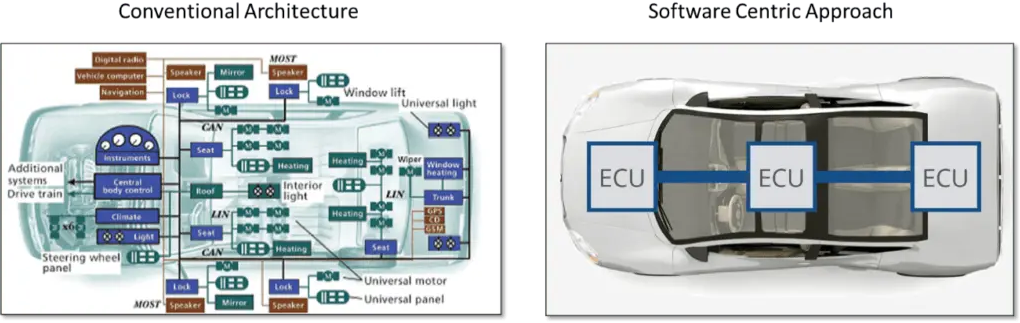
\includegraphics[width=1\textwidth]{centralized-architecture}
    \caption{Current and next-gen architecture of cars \cite{car-architecture}.}
    \label{fig:centralized-architecture}
\end{figure}

ECUs communicate with each other via bus systems. The most common ones are CAN(Controller Area Network), FlexRay and the Automotive Ethernet, which is becoming increasingly popular. Transport protocols sit on top of these physical layers. For Ethernet these are the well-known TCP or UDP protocols, while for CAN the ISO-TP protocol is the most common one.

Application protocols are used to ultimately transfer payload. Some protocols were created specifically for the development of units like the Universal Measurement and Calibration Protocol (XCP) and some others were defined for diagnostic related tasks, such as the Unified Diagnostic Services (UDS), General Motors Local Area Network (GMLAN) and On-board diagnostics (OBD). Both types are security critical. 
The XCP protocol is able to read and even write into the flash memory of an ECU. It shall be disabled on shipped ECUs.

However, diagnostic protocols are explicitly designed for actively used cars and thus exposed to the easily accessible OBD-II port (see \autoref{fig:obd-port}), which by regulation must be present near the steering wheel on at least every car built from 2003 onwards, making them a great source of information.
This thesis focuses on the UDS protocol, as it is the most widely used protocol that allows extended functionality, such as flashing ECUs. The OBD protocol is excluded because it does not provide valuable information, and the GMLAN protocol because it is limited to General Motors vehicles.

\begin{figure}[htb]
    \centering
    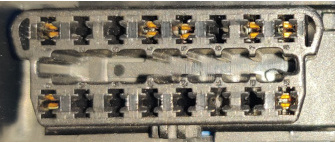
\includegraphics[width=0.5\textwidth]{obd-port}
    \caption{The OBD-II port of a BMW.}
    \label{fig:obd-port}
\end{figure}

The initial step in testing a system for weaknesses is to gather as much information from it as possible. In most cases, a protocol definition does not require that its specification is fully supported; instead, a subset is sufficient.
Furthermore, a diagnostic protocol can define various states. 
The ECU may show varying behaviors in different states, for example support for other services. Since this kind of information is highly relevant for the security of the ECU, it would be helpful for security testers to gain this knowledge quickly and automatically.

One option to achieve this is to send all possible requests to an ECU and evaluate the responses. In the context of the project \emph{Penetration Test Driven Safety and Security System Improvements for Cyber-Critical Systems} (PetS3) \cite{pets3} such scanners have been implemented for UDS, GMLAN and OBD.

With their brute-force approaches, they are effective but not efficient. A scan can take a highly variable amount of time. 
It can range from a few hours to a day or more. In general, the more states are found on an ECU in a scan, the more time it will need. For example, more authentication information lead to more state detections and thus to higher runtimes. In addition, the response time of the ECU is also a decisive factor. 
The original runtimes observed for a UDS scan on some ECUs are shown in \autoref{fig:durations}. It should be noted, that these scans have been executed with no additional information about the ECU as well. 
Accordingly, only the states that can be found without further information were detected (black-box test).

%durations
\begin{figure}[htb]
    \centering
    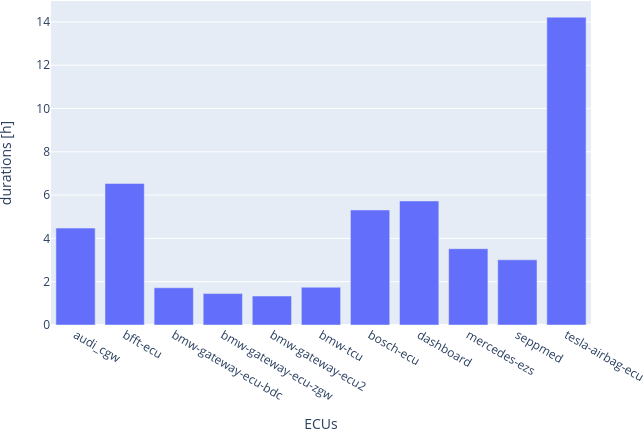
\includegraphics[width=0.8\textwidth]{durations}
    \caption{Observed runtimes for a UDS scan.}
    \label{fig:durations}
\end{figure}

Consequently, an efficient scan is important to keep the scan time low even though many states can be found or the ECU has a high response time.

\section{Goal}

This paper evaluates three approaches to improve the efficiency of the UDS protocol scanning, namely reusing information within the same service (approach 1), using probabilities of positive answers based on blocks (approach 2) and avoiding scanning unsupported services (approach 3).

The basic idea of all approaches is to reduce the number of requests where no positive response is expected.

Efficiency improvement is understood as the ratio between the request savings and the coverage. In this context, coverage is defined as the ratio of finds in the unmodified scanner to the finds of the modified scanner, and the request savings as the ratio of requests in comparison between these two. For both metrics, the higher the better.

Nevertheless, they have to be in balance. A request saving of 90\,\% is worth little if this results in 0\,\% coverage. Hence, the challenge is to narrow down the scanning area to where positive responses are expected.

In concrete terms, the following questions are to be answered:

\begin{itemize}
    \item How to apply the approaches for best results?
    \item What is the coverage for each approach?
    \item What is the request saving for each approach?
    \item Are the implementations of the approaches a replacement for the original implementations?
\end{itemize}


\section{Environment}
This work was created at eMundo GmbH in Ingolstadt. It is an IT service company which plans and executes projects for customers. Also, it is an aspiring company which in 20 years managed to open in total six company headquarters in Germany, Austria and Italy with almost 100 employees.

Since 2018, they are part of the PetS3 project that is a collaboration research project among the OTH Regensburg, TH Nürnberg, EDAG Engineering Group AG, sepp.med GmbH, intive automotive GmbH and eMundo GmbH. The aim of this project is to investigate the interactions between functional and IT security for system networks in cars \cite{pets3}.

This paper is the final result of this project on the part of eMundo.

\section{Outline}

First, Chapter 2 describes the basics for understanding this thesis. After that, Chapter 3 shows how and what data was collected for the analysis and how it was used for profiling the UDS Scanner. Chapter 4 then elaborates on the approaches based on the data collected.
Consequently, their implementation is explained in Chapter 5. The observed results of the implementations on ECUs are presented in Chapter 6. Finally, Chapter 7 summarizes the results of this thesis and provides an outlook on future work.
